\chapter{Metodología}\label{chapter:methods}

En este capítulo se describe detalladamente el proceso de


\section{Descripción CRISP-DM}

\section{Descripción del conjunto de datos}

El conjunto de datos está organizado en preguntas y respuestas de las categorías: Medicina, Enfermería, Bilogía, Química, Psicología, y Farmacología. Y está dividido en train, development y test. El datset está compuesto por un conjunto de preguntas/respuestas en formato JSON siguiendo la siguientes estructura:

\begin{itemize}
  \item Id: identificador y texto de la pregunta
  \item Ruta: camino a la imagen si lo hay
  \item Respuestas: Una lista con las posibles respuestas
  \item El id de la respuesta correcta
\end{itemize}


\section{Análisis del conjunto de datos}

\subsection{Análisis descriptivo}

\subsection{Procesamiento de datos}


\chapter{Modelos propuestos}\label{chapter:models}

\section{Regresión Logística}

El primer modelo a implementar es un regresor logístico. La simplicidad de este modelo lo hace un buen candidato para establecer un \textit{baseline} entre los modelos de aprendizaje supervisado.


\section{\textit{LSTM} Básico}\label{lstm_t}

La primera propuesta se puede considerar un modelo de aprendizaje profundo relativamente sencillo cuyo objetivo principal es verificar las ventajas que proporcionan las redes recurrentes en la resolución del problema de selección de respuestas. Por esta razón el modelo presentado aprovecha la arquitectura recurrente de la manera más simple posible.

La primera propuesta consiste en una red neuronal recurrente de tipo \textit{LSTM}, la cual recibe como entrada una oración vectorizada. La arquitectura se divide en tres capas: representación de los \textit{tokens}, representación de la oración y predicción de la etiqueta (respuesta correcta). En la Figura \ref{lstm} se presenta la arquitectura de la red correspondiente al modelo matemático que se expone a continuación.

\begin{figure}[!tb]
  \begin{center}    
    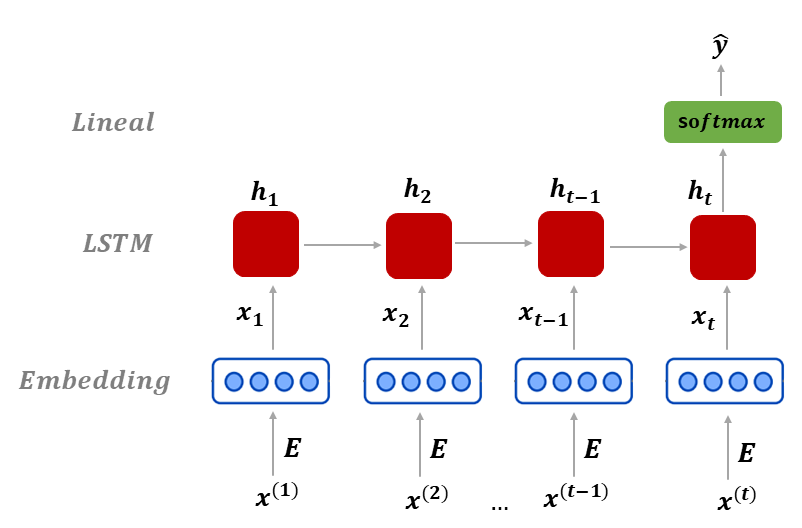
\includegraphics[angle=0, width=0.75\textwidth]{Graphics/lstm2.png} 
  \end{center}
    \caption{Arquitectura del modelo de extracción de relaciones LSTM básico}\label{lstm}
\end{figure}

Sea $S = [x^{(1)}, x^{(2)}, ..., x^{(T)}]$ la representación vectorial de una oración $S$, donde $x^{(t)}$ representa el t-ésimo \textit{token} con $(t = 1, 2, ..., T)$ y $T$, la cantidad de \textit{tokens} de la oración. El modelo puede ser definido formalmente como:

\begin{align}
  x_{t} &= Ex^{(t)} \label{lstm:emb} \\
  \nonumber \\
  i_{t} &= \sigma{(W^{(i)} x_{t} + U^{(i)}h_{t-1})} \label{lstm:ig} \\
  f_{t} &= \sigma{(W^{(f)} x_{t} + U^{(f)}h_{t-1})} \label{lstm:fg} \\
  o_{t} &= \sigma{(W^{(o)} x_{t} + U^{(o)}h_{t-1})} \label{lstm:og} \\
  \tilde{c_{t}} &= \tanh(W^{(c)} x_{t} + U^{(c)}h_{t-1}) \label{lstm:new_memory_generation} \\
  c_{t} &= f_{t}c_{t-1} + i_{t}\tilde{c_{t}} \label{lstm:cell_state} \\
  h_{t} &= o_{t}\tanh{c_{t}} \label{lstm:hidden_state} \\
  \nonumber \\
  \hat{y} &= softmax(Uh_{T} + b) \label{lstm:pred}
\end{align}

En una primera etapa (Ecuación \ref{lstm:emb}), el modelo obtiene una representación más rica semánticamente de cada uno de los \textit{tokens} que conforman una oración. Esto se logra a través de una capa de \textit{embeddings} $E$ que transforma cada \textit{token} $x^{(t)}$ en un vector $x_{t}$ $\in$ ${\mathbb{R}} ^{d}$, donde $d$ es la dimensión de los \textit{embeddings} que constituye un hiperparámetro del modelo.

En la segunda etapa (Ecuaciones \ref{lstm:ig} - \ref{lstm:hidden_state}), el modelo procesa la secuencia de \textit{tokens} para obtener una representación final de la oración. Esto se logra con la inclusión de una capa \textit{LSTM}, la cual analiza de manera secuencial cada una de las salidas $x_{t}$ de la capa de \textit{embeddings}. El centro de una red \textit{LSTM} es el funcionamiento de sus celdas, una red \textit{LSTM} tiene tantas celdas como \textit{tokens} tiene una oración. Las Ecuaciones \ref{lstm:ig} - \ref{lstm:hidden_state} describen el comportamiento de una celda de la red \textit{LSTM}. En la tabla \ref{tab:cell_state} se describe la notación empleada.

\begin{table}[!tb]
  \center \caption{Descripción de símbolos utilizados en una red \textit{LSTM}}
    \begin{center}
      \begin{tabular}{|c|l|}
        \hline
        \textbf{Símbolo} & \textbf{Significado}\\
        \hline
        $x_{t}$ & entrada a la celda \textit{LSTM} en el paso $t$ \\
        $h_{t-1}$ & salida de la celda \textit{LSTM} en el paso $t-1$ \\
        $i_{t}$ & valor de la \textit{input gate} en el paso $t$\\
        $f_{t}$	& valor de la \textit{forget gate} en el paso $t$ \\
        $o_{t}$	& valor de la \textit{output gate} en el paso $t$\\
        $\sigma$ & función sigmoidal\\
        $W^{(\alpha)}$ & pesos de $x_{t}$ en $\alpha_t$ ($\alpha = {i, f, o}$) \\
        $U^{(\alpha)}$ & pesos de $h_{t-1}$ en $\alpha_t$ ($\alpha = {i, f, o}$) \\
        $\tilde{c_{t}}$ & candidato a \textit{cell state} en el paso $t$\\
        $c_{t}$ & \textit{cell state} en el paso $t$ \\
        $h_{t}$ & salida final de la celda \textit{LSTM} en el paso $t$ \\
        $h_{T}$ & salida final de la celda \textit{LSTM} en el último paso $T$ \\
        \hline
        \end{tabular}
    \end{center}
    \label{tab:cell_state}
\end{table}

Una celda \textit{LSTM} está compuesta por tres componentes fundamentales:
\begin{itemize}
  \item La \textit{input gate}, en español "válvula de entrada", expresada en la Ecuación \ref{lstm:ig}, tiene la función de determinar qué información debe estar presente en el estado de la celda (en inglés, \textit{cell state}) representado por $c_{t}$, teniendo en cuenta la salida final de la celda anterior $h_{t-1}$.
  \item La \textit{forget gate}, en español "válvula del olvido", representada en la Ecuación \ref{lstm:fg}, tiene la función de determinar qué información es irrelevante en el estado de la celda $c_{t}$; funciona de manera análoga a la \textit{input gate}.
  \item La \textit{output gate}, en español "válvula de salida", representada en la Ecuación \ref{lstm:og}, tiene la función de determinar el nivel de activación del estado $c_{t}$ para la salida final.
\end{itemize}

En todos estos casos, se utiliza como función de activación la función sigmoide $\sigma$ con el propósito de que los valores sean positivos y se encuentren entre 0 y 1; de esa manera es sencillo interpretar la importancia de las componentes.

La Ecuación \ref{lstm:new_memory_generation}, conocida como \textit{new memory generation} o \textit{candidate cell}, calcula un estado recurrente temporal $\tilde{c_{t}}$ teniendo en cuenta la entrada $x_{t}$ y el estado anterior $h_{t-1}$. En este caso, para superar el problema de \textit{vanishing gradient}\footnote{https://towardsdatascience.com/the-vanishing-gradient-problem-69bf08b15484} se necesita una función de activación cuya segunda derivada pueda mantenerse durante un largo rango antes de llegar a cero, razón por la cual se utiliza la tangente.

En la Ecuación \ref{lstm:cell_state} se calcula el estado de la celda actual $c_{t}$ teniendo en cuenta qué debe olvidar del estado previo a través de la expresión $f_{t}*c_{t-1}$ y qué debe considerar del estado actual temporal representado en la expresión $i_{t}*\tilde{c_{t}}$. En la Ecuación \ref{lstm:hidden_state} se toma el estado de la celda $c_{t}$ y la \textit{output gate} $o_{t}$ para determinar qué información queda contenida en el estado último de la celda $h_{t}$.

Es importante destacar que los parámetros $E$, $W^{(i)}$, $W^{(f)}$, $W^{(o)}$, $W^{(c)}$, $U^{(i)}$, $U^{(f)}$, $U^{(o)}$, $U^{(c)}$ y $U$ son aprendidos durante la etapa de entrenamiento en el proceso de \textit{backpropagation}.

Las operaciones presentadas en las ecuaciones \ref{lstm:ig} - \ref{lstm:hidden_state} son ejecutadas $T$ veces, por cada uno de los \textit{tokens} que conforman una oración. Tras el análisis del último \textit{token} $T$, el estado final $h_{T}$ constituye una representación de la oración $S$. Finalmente, una capa lineal (Ecuación \ref{lstm:pred}) utiliza la representación de la oración obtenida $h_{T}$ para predecir la relación $\hat{y}$ existente en la oración. Esta salida se convierte en una distribución de probabilidades empleando la función \textit{softmax}. Esta operación, a diferencia de las ecuaciones anteriores, solo se aplica una vez al estado final $h_{T}$ de la capa \textit{LSTM}.

La sencillez arquitectónica del modelo permite que se pueda utilizar como base para la comparación con otros modelos más complejos que serán abordados a continuación.

\section{\textit{Transfer Learning} basado en BERT}\label{bert_t}

\cite{2018-devlin-bert} plantea que el uso de BERT en el enfoque \textit{fine tuning} obtiene nuevos resultados en el estado del arte en varias tareas de procesamiento del lenguaje natural, entre ellas, el reconocimiento de entidades nombradas y los sistemas pregunta/respuesta.

La diferencia con otros modelos de representación del lenguaje, en cuanto a arquitectura, es que BERT está basado en un \textit{Transformer} bidireccional. En el artículo de \cite{2018-devlin-bert} no se detalla la arquitectura del modelo \textit{Transformer}. Otra diferencia es que modifica la tarea tradicional de \textit{language modeling} sobre la que se entrena introduciendo nuevas tareas. La primera tarea introducida recibe el nombre de \textit{masked language model} y consiste en ocultar palabras aleatorias en un texto y predecir, teniendo en cuenta el contexto, el \textit{token} que corresponde a la posición oculta, mientras que la segunda tarea consiste en, dada una oración en un texto, predecir la oración siguiente.

Los autores de BERT señalan como principal contribución la demostración de la efectividad del pre-entrenamiento bidireccional en la representación del lenguaje sobre las arquitecturas unidireccionales utilizadas hasta ese momento y, además, plantean que con el uso de esta nueva representación se puede reducir la complejidad de la arquitectura del modelo y aún así, obtener mejores resultados.

En esta tesis se propone un modelo que hace uso del modelo de lenguaje aprendido utilizando BERT e incorpora un modelo de predicción simple. La propuesta tiene como objetivo comprobar si los aportes de BERT se pueden extender al idioma español y, específicamente, a la tarea de extracción de relaciones semánticas entre entidades.

\subsection{Especificidad del preprocesamiento}

Con el objetivo de transformar una oración en un vector computacionalmente interpretable, se propuso un preprocesamiento que fue aplicado a los modelos de aprendizaje presentados. Sin embargo, en el caso de BERT, las oraciones no pueden ser traducidas a vectores numéricos de la misma forma que se hizo en las propuestas anteriores, sino que BERT requiere un formato diferente. Con el fin de obtener los resultados esperados, el corpus original siempre debe ser modificado en función de las pautas planteadas por los autores en \cite{2018-devlin-bert}.

BERT define los siguientes \textit{tokens} especiales para la representación de una oración. Dichos \textit{tokens} reciben una interpretación diferente en la etapa de entrenamiento.
\begin{itemize}
  \item \textbf{[CLS]}: Indica el inicio de una oración
  \item \textbf{[SEP]}: Indica el fin de una oración
  \item \textbf{[MASK]}: Se utiliza para denotar \textit{tokens} que deben ser ignorados por el modelo
\end{itemize}

BERT no acepta secuencias de tamaño variable por lo que se recurre a la estrategia de \textit{padding}, en la que se establece un tamaño máximo. Las oraciones que tienen una cantidad menor de \textit{tokens} son completadas con el \textit{token} especial \textbf{[MASK]}, para indicar que esas posiciones deben ser ignoradas.

\section{Implementación}




